\documentclass[14pt,a4paper,report]{report}
\usepackage[a4paper, mag=1000, left=2.5cm, right=1cm, top=2cm, bottom=2cm, headsep=0.7cm, footskip=1cm]{geometry}
\usepackage[utf8]{inputenc}
\usepackage[english,russian]{babel}
\usepackage{indentfirst}
\usepackage[dvipsnames]{xcolor}
\usepackage[colorlinks]{hyperref}
\usepackage{listings} 
\usepackage{fancyhdr}
\usepackage{caption}
\usepackage{amsmath}
\usepackage{latexsym}
\usepackage{graphicx}
\usepackage{amsmath}
\usepackage{booktabs}
\usepackage{array}
\hypersetup{
	colorlinks = true,
	linkcolor  = black
}

\usepackage{titlesec}
\titleformat{\chapter}
{\Large\bfseries} % format
{}                % label
{0pt}             % sep
{\huge}           % before-code


\DeclareCaptionFont{white}{\color{white}} 

% Listing description
\usepackage{listings} 
\DeclareCaptionFormat{listing}{\colorbox{gray}{\parbox{\textwidth}{#1#2#3}}}
\captionsetup[lstlisting]{format=listing,labelfont=white,textfont=white}
\lstset{ 
	% Listing settings
	inputencoding = utf8,			
	extendedchars = \true, 
	keepspaces = true, 			  	 % Поддержка кириллицы и пробелов в комментариях
	language = Matlab,            	 	 % Язык программирования (для подсветки)
	basicstyle = \small\sffamily, 	 % Размер и начертание шрифта для подсветки кода
	numbers = left,               	 % Где поставить нумерацию строк (слева\справа)
	numberstyle = \tiny,          	 % Размер шрифта для номеров строк
	stepnumber = 1,               	 % Размер шага между двумя номерами строк
	numbersep = 5pt,              	 % Как далеко отстоят номера строк от подсвечиваемого кода
	backgroundcolor = \color{white}, % Цвет фона подсветки - используем \usepackage{color}
	showspaces = false,           	 % Показывать или нет пробелы специальными отступами
	showstringspaces = false,    	 % Показывать или нет пробелы в строках
	showtabs = false,           	 % Показывать или нет табуляцию в строках
	frame = single,              	 % Рисовать рамку вокруг кода
	tabsize = 2,                  	 % Размер табуляции по умолчанию равен 2 пробелам
	captionpos = t,             	 % Позиция заголовка вверху [t] или внизу [b] 
	breaklines = true,           	 % Автоматически переносить строки (да\нет)
	breakatwhitespace = false,   	 % Переносить строки только если есть пробел
	escapeinside = {\%*}{*)}      	 % Если нужно добавить комментарии в коде
}

\begin{document}

\def\contentsname{Содержание}

% Titlepage
\begin{titlepage}
	\begin{center}
		\textsc{Санкт-Петербургский Политехнический 
			Университет Петра Великого\\[5mm]
			Кафедра компьютерных систем и программных технологий}
		
		\vfill
		
		\textbf{Отчёт по дополнительному заданию\\[3mm]
			Курс: «Методы оптимизации и принятия решений»\\[3mm]
			Тема: «Проверка расчетов»\\[35mm]
			}
	\end{center}
	
	\hfill
	\begin{minipage}{.5\textwidth}
		Выполнил студент:\\[2mm] 
		Бояркин Никита Сергеевич\\
		Группа: 13541/3\\[5mm]
		
		Проверил:\\[2mm] 
		Сиднев Александр Георгиевич
	\end{minipage}
	\vfill
	\begin{center}
		Санкт-Петербург\\ \the\year\ г.
	\end{center}
\end{titlepage}

% Contents
\tableofcontents
\clearpage

\chapter{Дополнительное задание}

\section{Ход работы}

\subsection{Формулировка задачи}

\begin{figure}[h!]
	\centering
	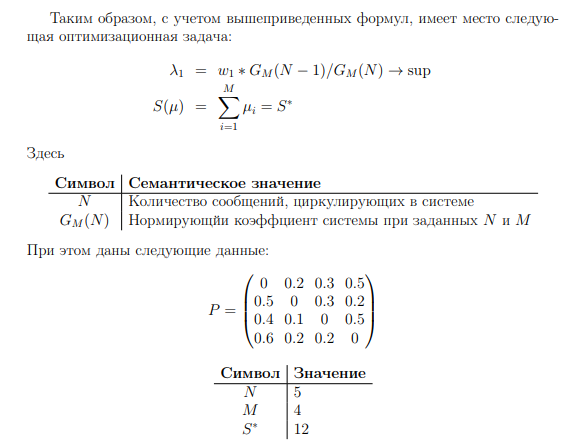
\includegraphics[scale = 1.01]{images/1.png}
	\label{image:1}
\end{figure}

\subsection{Решение для проверки}

Данное решение необходимо проверить:

\begin{figure}[h!]
	\centering
	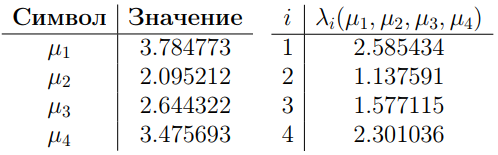
\includegraphics[scale = 0.8]{images/2.png}
	\label{image:2}
\end{figure}

\subsection{Решение задачи через нормирующую константу методом Ньютона}

Решение задачи через нормирующую константу методом Ньютона c начальным приближением $u=[3, 3, 3, 3]$ и значением ошибки $e=1e^{-8}$:

\lstinputlisting{listings/l3.m}

Расчет нормирующей константы:

\lstinputlisting{listings/gl3.m}

Расчет основных характеристик СМО:

\lstinputlisting{listings/pl3.m}

Результат решения задачи методом Ньютона  c начальным приближением $u=[3, 3, 3, 3]$ и значением ошибки $e=1e^{-8}$:

\lstinputlisting{listings/l3.log}

Алгоритм успешно сходится за 7 итераций. С каждой итерацией алгоритма значения целевых функций стемятся к нулю.

\begin{table}[h!]
	\centering
	\bgroup
	\captionsetup{singlelinecheck = false, format= hang, justification=raggedleft, font=footnotesize, labelsep=space}
	\caption{Сравнительный анализ решений}
	\def\arraystretch{1}
	\begin{tabular}{ | m{0.21cm} | m{1.25cm} | m{1.25cm} | m{1.25cm} | m{1.25cm} | m{1.25cm} | m{1.25cm} |}
		\hline
		$i$ & $\mu_{task}(i)$ & $|\mu_{my}(i)|$ & $\Delta\mu(i)$ & $\lambda_{task}(i)$ & $\lambda_{my}(i)$ & $|\Delta\lambda(i)|$ \\ \hline
		1 & 3.784773 & 3.781633 & 0.00314 & 2.585434 & 2.582525 & 0.002909 \\ \hline
		2 & 2.095212 & 2.092512 & 0.0027 & 1.137591 & 1.135533 & 0.002058 \\ \hline
		3 & 2.644322 & 2.643885 & 0.000437 & 1.577115 & 1.576768 & 0.000347 \\ \hline
		4 & 3.475693 & 3.481970 & 0.006277 & 2.301036 & 2.306753 & 0.005717 \\
		\hline
	\end{tabular}
	\egroup
\end{table}


\section{Вывод}

Решение сошлось с заданным до третьего знака после запятой. Небольшая погрешность объясняется различием в алгоритме расчета нормирующей константы G, а также вычислением при помощи различных языков программирования (R и Matlab). 

\end{document}